%%%------------------------------------------------------------------------------------------------------------
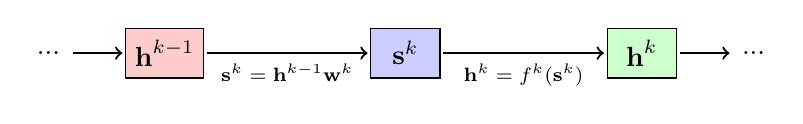
\begin{tikzpicture}
\begin{scope}
\node [anchor=center,draw,fill=red!20,minimum height=1.8em,minimum width=2.5em] (h) at (0,0) {$\textbf{h}^{k-1}$};
\node [anchor=west,draw,fill=blue!20,minimum height=1.8em,minimum width=2.5em] (s) at ([xshift=6em]h.east) {$\textbf{s}^{k}$};
\node [anchor=west,draw,fill=green!20,minimum height=1.8em,minimum width=2.5em] (h2) at ([xshift=6em]s.east) {$\textbf{h}^{k}$};
\node [anchor=east] (prev) at ([xshift=-2em]h.west) {...};
\node [anchor=west] (next) at ([xshift=2em]h2.east) {...};
\draw [->,thick] ([xshift=0.1em]prev.east) -- ([xshift=-0.1em]h.west);
\draw [->,thick] ([xshift=0.1em]h.east) -- ([xshift=-0.1em]s.west) node [pos=0.5,below] {\scriptsize{$\textbf{s}^k = \textbf{h}^{k-1}\textbf{w}^k$}};
\draw [->,thick] ([xshift=0.1em]s.east) -- ([xshift=-0.1em]h2.west) node [pos=0.5,below] {\scriptsize{$\textbf{h}^k = f^k(\textbf{s}^{k})$}};
\draw [->,thick] ([xshift=0.1em]h2.east) -- ([xshift=-0.1em]next.west);


\end{scope}
\end{tikzpicture}
%%%------------------------------------------------------------------------------------------------------------

